\documentclass[10pt]{article}
\usepackage{amsmath,amssymb,amsthm}
\usepackage[margin=0.6in]{geometry} 
\usepackage{enumitem} 
\usepackage{fancyhdr}
\usepackage{tikz} 

% --- Page Style Setup ---
\pagestyle{fancy}
\fancyhead{} 
\fancyfoot[R]{\thepage} 
\fancyfoot[C]{Sorting Algorithms Practice} 
\renewcommand{\headrulewidth}{0pt} 

% Set spacing: No paragraph skip and no paragraph indent
\setlength{\parskip}{0pt}
\setlength{\parindent}{0pt}

% Define a consistent height for fill-in-the-blank answers 
\newcommand{\answerbox}[1]{\parbox[t]{0pt}{\vspace{#1}}} 

\begin{document}
\begin{center}
    {\small \textbf{IA Competitive Programming Club}} \\[6pt]
    {\Large Sorting Worksheet} \\[12pt]
    {\small November 12, 2025}
\end{center}
\thispagestyle{fancy} 

% ----------------------------------------------------------------------
% Section I: Core Mechanics and Time Complexity
% ----------------------------------------------------------------------
\section*{Part I: Core Mechanics and Time Complexity}
\hrule
\vspace{0.2cm} % Slightly reduced space here

% Reduced itemsep slightly for compactness
\begin{enumerate}[label=\textbf{Q\arabic*.}, leftmargin=*, itemsep=1.2cm] 

    \item \textbf{Best-Case Efficiency}
    Which of the three algorithms (\textbf{Bubble}, \textbf{Insertion}, \textbf{Selection}) has $\mathcal{O}(N)$ time when the array is already sorted?
    
    \answerbox{1.4cm} % Slight reduction

    \item \textbf{Counting Swaps}
    In which algorithm is the number of swaps always $\mathcal{O}(N)$ in the worst case?
    
    \answerbox{1.4cm} % Slight reduction

    \item \textbf{Trace: Selection Sort}
    Show the array after the first two passes on the initial array:
    \[
    [9, 1, 5, 2, 4]
    \]
    % Inner list for sub-questions
    \begin{enumerate}[label=\alph*., leftmargin=1cm, itemsep=0.6cm] % Slight reduction
        \item After 1st pass: \underline{\hspace{6cm}} 
        \item After 2nd pass: \underline{\hspace{6cm}}
    \end{enumerate}
    
    \item \textbf{Big-$\mathcal{O}$ Comparison}
    Fill in the Big-$\mathcal{O}$ complexities.
    \begin{center}
    \renewcommand{\arraystretch}{1.3} % Slightly reduced row height
    \begin{tabular}{|l|c|c|}
        \hline
        \textbf{Algorithm} & \textbf{Best Case} & \textbf{Worst Case} \\
        \hline
        Bubble Sort & \answerbox{0.4cm} & \answerbox{0.4cm} \\
        \hline
        Insertion Sort & \answerbox{0.4cm} & \answerbox{0.4cm} \\
        \hline
        Selection Sort & \answerbox{0.4cm} & \answerbox{0.4cm} \\
        \hline
    \end{tabular}
    \end{center}
\end{enumerate}

% ----------------------------------------------------------------------
% Section II: Visualization and Practice
% ----------------------------------------------------------------------
\newpage 
\section*{Part II: Visualization and Practice}
\hrule
\vspace{0.2cm} % Slightly reduced space here

\subsection*{Problem 5: Insertion Sort Visualization}
\textbf{Problem:} The diagram shows an array during \textbf{Insertion Sort}. Gray = sorted portion.

\begin{center}
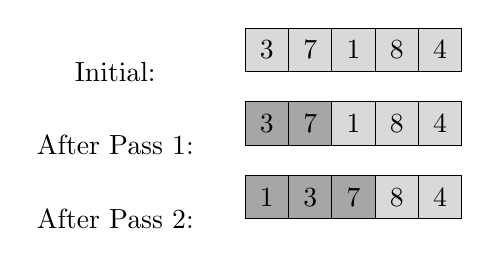
\begin{tikzpicture}[scale=0.55] 
    % --- Initial ---
    \node at (-1.5, 0) {Initial:}; % Removed \hspace{...}
    \foreach \i / \val in {0/3,1/7,2/1,3/8,4/4}{
        \pgfmathsetmacro{\xstart}{\i+1.5} % SHIFTED X by +1.5
        \pgfmathsetmacro{\xmid}{\i+2.0}   % SHIFTED X by +1.5
        \draw[fill=gray!30](\xstart,0)rectangle(\xstart+1,1);
        \node at(\xmid,0.5){\val};
    }
    
    % --- After Pass 1 ---
    \node at (-1.5,-1.7){After Pass 1:}; % Removed \hspace{...}
    \foreach \i / \val in {0/3,1/7,2/1,3/8,4/4}{
        \pgfmathsetmacro{\shade}{ifthenelse(\i<=1,70,30)}
        \pgfmathsetmacro{\xstart}{\i+1.5} % SHIFTED X by +1.5
        \pgfmathsetmacro{\xmid}{\i+2.0}   % SHIFTED X by +1.5
        \draw[fill=gray!\shade](\xstart,-1.7)rectangle(\xstart+1,-0.7);
        \node at(\xmid,-1.2){\val};
    }
    
    % --- After Pass 2 ---
    \node at (-1.5,-3.4){After Pass 2:}; % Removed \hspace{...}
    \foreach \i / \val in {0/1,1/3,2/7,3/8,4/4}{
        \pgfmathsetmacro{\shade}{ifthenelse(\i<=2,70,30)}
        \pgfmathsetmacro{\xstart}{\i+1.5} % SHIFTED X by +1.5
        \pgfmathsetmacro{\xmid}{\i+2.0}   % SHIFTED X by +1.5
        \draw[fill=gray!\shade](\xstart,-3.4)rectangle(\xstart+1,-2.4);
        \node at(\xmid,-2.9){\val};
    }
\end{tikzpicture}
\end{center}

\textbf{Task:} Draw or describe the array after inserting ‘8’ (next pass).
\answerbox{1.8cm} % Slight reduction

\subsection*{Problem 6: Swap Counting (Bubble Sort)}
\textbf{Input:} $A = [4, 1, 3, 2]$
\textbf{Task:}
\begin{enumerate}[label=(\alph*), itemsep=0.8cm, leftmargin=1cm] % Slight reduction
    \item Show array after first two full passes.
    \answerbox{2.2cm} % Slight reduction

    \item Total number of swaps to fully sort?
    \answerbox{1.0cm} % Slight reduction
\end{enumerate}

% ---------------------------------
% Remaining Problems
% ---------------------------------

\subsection*{Problem 7: Modifying Sorting Direction}
To sort in \textbf{descending} order:
\begin{enumerate}[label=(\alph*), itemsep=0.8cm, leftmargin=1cm] % Slight reduction
    \item In \textbf{Insertion Sort}, which comparison operator changes, and how?
    \answerbox{1.1cm} % Slight reduction

    \item In \textbf{Selection Sort}, do we find the minimum or maximum each pass?
    \answerbox{1.3cm} % Slight reduction
\end{enumerate}

\subsection*{Problem 8: Efficiency on Sorted Input}
For $B = [1,2,3,4,5,6,7,8,9,10]$:
\begin{enumerate}[label=(\alph*), itemsep=0.8cm, leftmargin=1cm] % Slight reduction
    \item About how many total comparisons does \textbf{Selection Sort} make (for $N=10$)?
    \answerbox{1.3cm} % Slight reduction

    \item For optimized \textbf{Bubble Sort} (stops if no swaps), how many passes and comparisons occur?
    \answerbox{1.3cm} % Slight reduction
\end{enumerate}

\end{document}